\chapter{Developing Data Acquisition Systems using new WEB Technologies}
\label{chap:III-2-web-daq}

  In the past years, web technologies have evolved to the point that fully fledged applications can be developed. The main advantage of these applications is that they can run on any platform and do not require installation processes by the client. \\

  In this chapter, we describe the architecture of a system making use of a MicroBlaze processor to run a web server and enable real-time communication between the front-end electronics and the control and monitoring application.

  \section{The Experimental Setup and System Architecture}

    The system is composed of the Xilinx SP601 development board to which the VFAT2 FMC is attached and connected to a VFAT2 Hybrid. Figure \ref{fig:III-2-sp601} is a photograph of the board showing the various components: the FPGA in the middle, the SDRAM on its right, the Ethernet connector and MAC controller in the bottom left corner, and the FMC connector on the left. The SP601 communicates with any computer on the network through an Ethernet connection. \\

    \begin{figure}[h!]
      \centering
      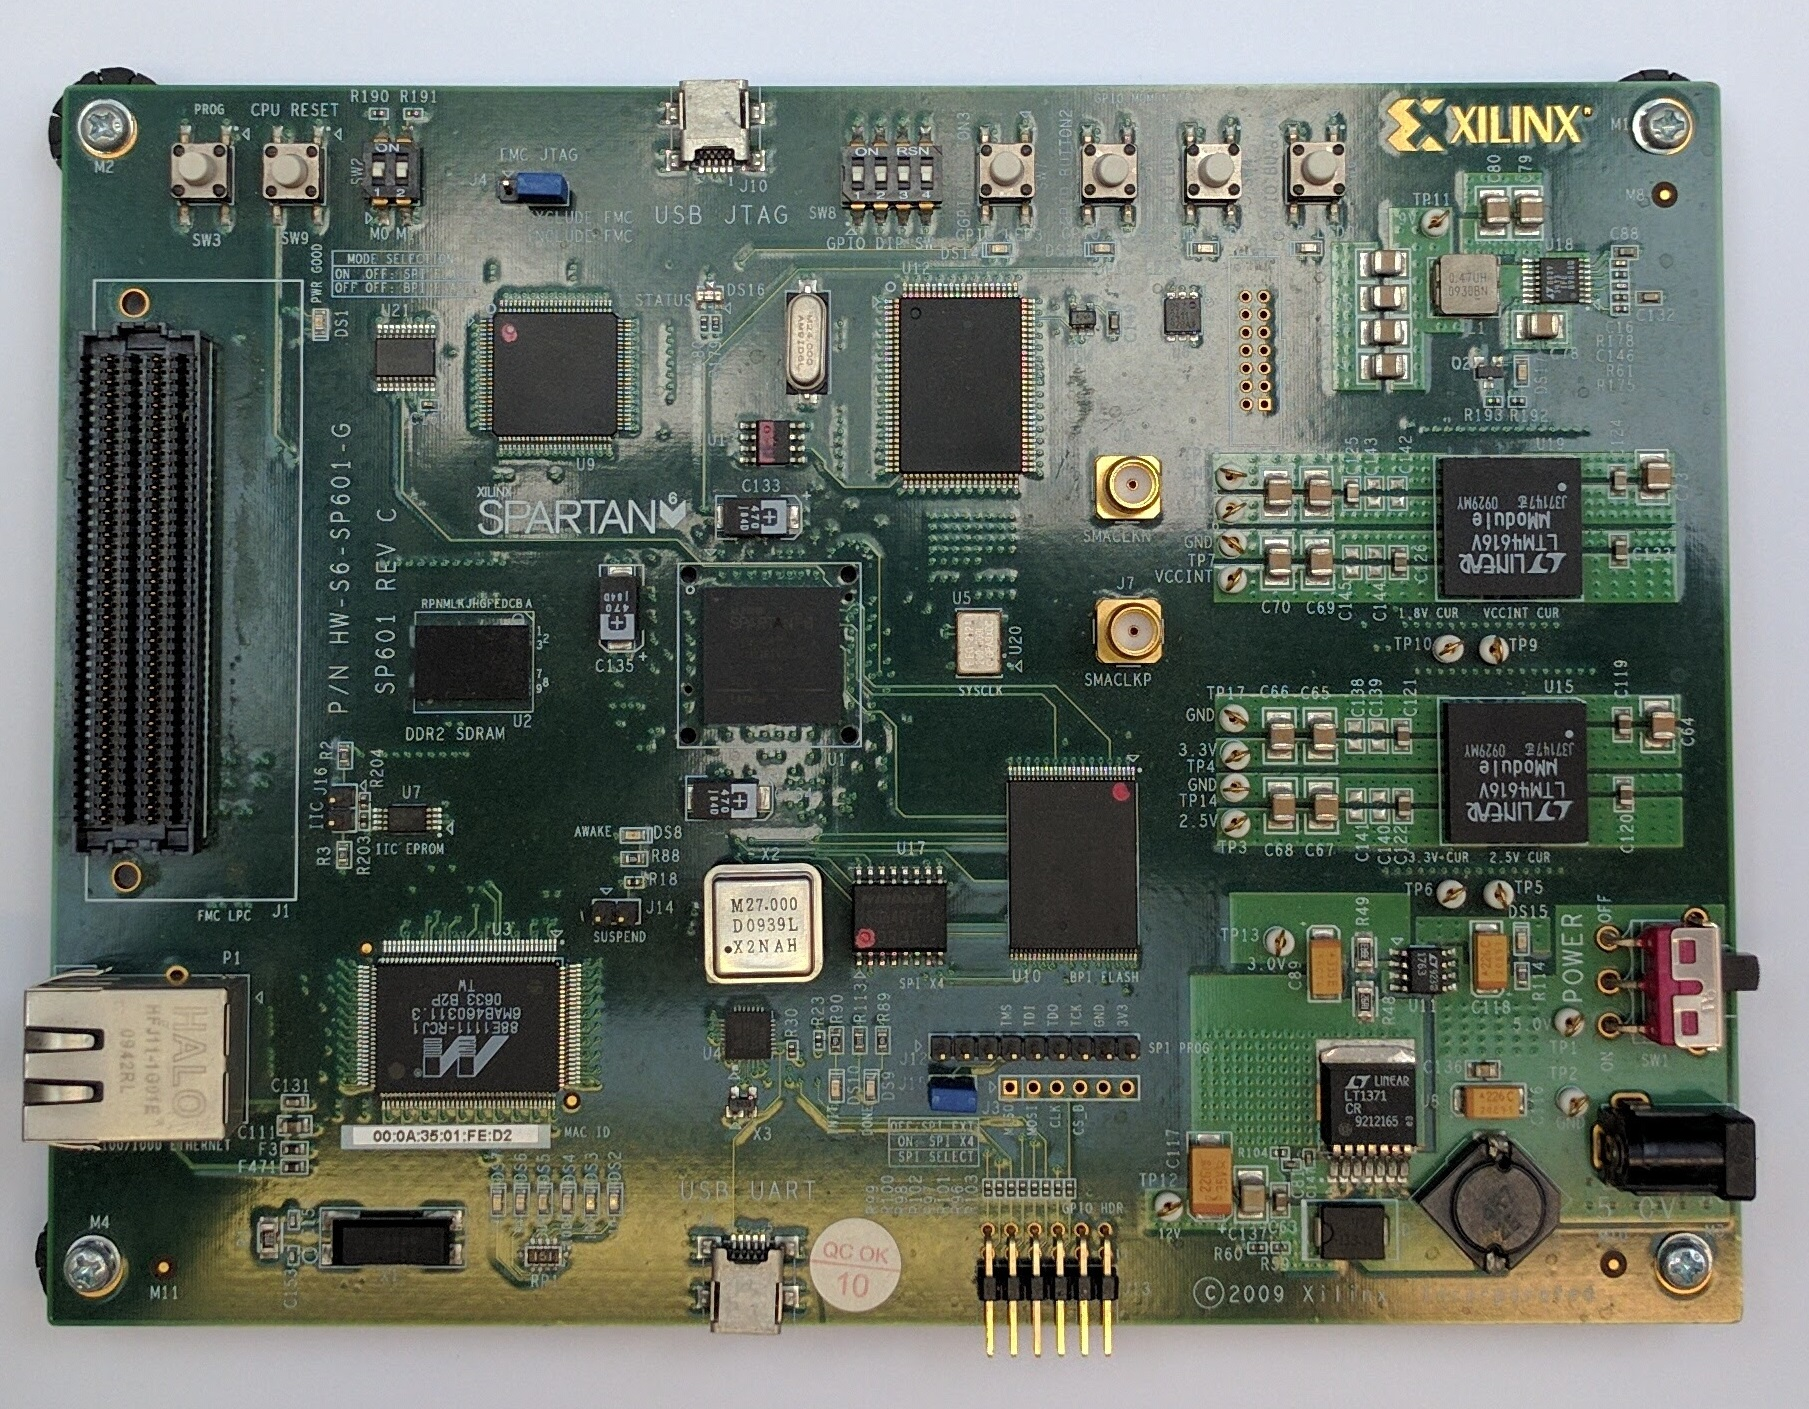
\includegraphics[width=0.8\textwidth]{img/III-2-web-daq/sp601.jpg}
      \caption{SP601}
      \label{fig:III-2-sp601}
    \end{figure}

    On the FPGA of the SP601, a dual-core Microblaze processor is implemented: one core handles the Ethernet connection and the other the communication with the VFAT2. The former runs a web server on top of the TCP/IP protocol in order to deliver the content of the web application used by the client to control and monitor the system ; the latter receives commands from the client and transfers them to the VFAT2. The whole system is contained in one board which can connect to various clients at the same time or to an external storage unit.

  \section{Web Server and WebSockets}

    A MicroBlaze processor is embedded on the FPGA of the SP601 and acts as web server to deliver web applications to clients which connect to the IP address of the board. Once the web application has been downloaded by the client, real-time communication is established over WebSockets to transmit requests between parties.

    \subsection{The HTTP Standard}

      When an internet browser pulls a web page from a server, it sends an Hypertext Transfer Protocol (HTTP) request containing the type of request and the path of the page. The type of request defines what the action of the client is. It can be GET, PUT, DELETE, etc which will respectively ask for a specific page, transfer content, delete content, etc. The path on the other hand can be a reference to a file to download, to a script to handle the new data, etc. The request is encoded in ASCII characters and is thus human-readable. Figure \ref{fig:III-2-http} displays an example of HTTP request and response in which the client requests a specific page and the server returns the content of that page. \\

      \begin{figure}[h!]
        \begin{tabularx}{\textwidth}{C{1}C{1}}
          \textbf{HTTP request} & \textbf{HTTP response} \\
        { \footnotesize
\begin{alltt}
\textcolor{blue}{GET} \textcolor{MidnightBlue}{/index.html} \textcolor{Plum}{HTTP/1.1} \newline
Host: www.web-daq.com
\end{alltt} } & { \footnotesize
\begin{alltt}
\textcolor{Plum}{HTTP/1.1} \textcolor{LimeGreen}{200 OK} \newline
Date: Thu, 28 July 2016 10:36:02 GMT \newline
Content-Type: text/plain; charset=UTF-8 \newline
Content-Encoding: UTF-8 \newline
Content-Length: 29 \newline
\textbf{This is the web application !}
\end{alltt} }
        \end{tabularx}
        \caption{}
        \label{fig:III-2-http}
      \end{figure}

      After analyzing the HTTP request, the server performs the desired operation and returns a status code, information headers, and optionally data. The status codes are defined in the HTTP standard: 200 means the operation was successful, 404 means that the request file is missing, 500 means the server encountered an error, etc. The additional headers contain information regarding the type of content that is returned (text, image, etc), the encoding of the data, the data size, etc. Finally, the response ends with the raw data. \\

      To each request, a single response is provided by the server. Moreover, the server does not initiate requests, meaning the communication has to be started by the client. The server can not push data to the client, but only provided data when probed (pulled).

    \subsection{The WebSocket Protocol}

      To allow the server to push data and enable real-time communication, the WebSocket standard was developed. WebSockets are sockets that can be used inside the internet browser to communicate with a server following a given data format. When a connection is established, it remains open on both sides reducing the overhead on each data packet and decreasing the latency. \\

      Upon connection from a client to the server, a dedicated HTTP request is sent informing the latter that the WebSocket protocol is being used. The server stores the information of the client in a list of active users until the latter disconnects or the connection times out. After this handshaking procedure, data can be sent between parties without restriction.

    \subsection{Handling Client Requests}

      The server on the MicroBlaze processor handles both HTTP and WebSocket requests, differentiating them using the HTTP header as selection criteria. It them forwards them to two dedicated functions according to the type of request. \\

      For HTTP requests, the headers are extracted along with the type and path. Only GET requests need to be handled in this application, corresponding to the download of resources: web page, image, etc. In case the path is valid, the file is retrieved from memory and sent back to the user. Otherwise, an error 404 is generated to inform the user that the resource is not available. In normal operation mode, the client connects once to the server over HTTP to download the application and then switches over to WebSocket communication. \\

      Once the application is downloaded, the connection with the server over WebSockets is established automatically. The server registers the client and real-time communication between parties can begin. Additionally, the server can establish a connection with a storage element to forward all events and log them in a database.

  \section{The MicroBlaze Processor}



    \subsection{Memory File System}

    \subsection{LWIP}

    \subsection{Dual Processor Architecture}

  \section{Conclusion}
